\section{Tecnologías}

\subsection{Lenguajes}

Como ya se ha hablado en varias ocasiones a lo largo de la memoria de los
lenguajes empleados, se remite al lector a las secciones \ref{sec:tecnologias}
y \ref{sec:diseno_del_sistema} para conocer las motivaciones de la elección de
PHP y el modo en que se ha empleado en el sistema.

A modo de introducción para el lector no iniciado (y con el deseo de que sean
unos pocos), \textbf{PHP} es un lenguaje de programación interpretado --en
contraste con los compilados-- especialmente útil para el desarrollo web del
lado del servidor, de manera que es muy usado en la programación de webs
dinámicas, delimitando el código PHP mediante los delimitadores
\verb|<?php| y \verb|?>|. Así, una primera aproximación sería:

\begin{lstlisting}
<!DOCTYPE html>
<html>
  <head>
    <meta charset="utf-8" />
    <title>Pruebe PHP</title>
  </head>
  <body>
  <?php
  echo 'Hola Mundo';
  /* echo("Hola Mundo"); tambien funciona,
  pero echo no es una funcion, sino un
  constructor del lenguaje. */
  ?>
  </body>
</html>
\end{lstlisting}

\textbf{JavaScript} también es un lenguaje de programación interpretado. Se
define como orientado a objetos, basado en prototipos, imperativo, débilmente
\textit{tipado} y dinámico. Uno de sus uso principales es el que se le ha dado
en este proyecto, para mejorar la experiencia del usuario al interactuar con la
interfaz. Como se explicará más adelante, también es crucial en la técnica de
desarrollo web Ajax, empleada en el buscador global. De nuevo, a modo de
simplísima introducción:

\begin{lstlisting}
<!DOCTYPE html>
<html>
  <head>
    <meta charset="utf-8" />
    <title>Pruebe JavaScript</title>
  </head>
  <body>
    <script type="text/javascript">
      document.write('Hola Mundo');
    </script>
    <noscript>
      <p>Su navegador no tiene soporta para JavaScript, 
      o este esta deshabilitado.</p>
    </noscript>
  </body>
</html>
\end{lstlisting}

A parte de PHP JavaScript, se ha hecho uso, por supuesto, de HTML, el lenguaje
de marcas predominante para la construcción de páginas web, así como de CSS
para la definición de los estilos del formato.

\subsection{Ajax}
\label{sec:fundamentos_ajax}

Ajax se utiliza para la creación de webs dinámicas y rápidas, permitiendo la
transferencia de información con el servidor de manera transparente para el
usuario, es decir, sin que este tenga que recargar la página. Su uso en la
actualidad está muy extendido en aplicaciones con alto grado de dinamicidad,
como Google Maps o Facebook.

Ajax está basado en estándares de Internet, y para su funcionamiento (figura
\ref{fig:ajax}) usa una combinación de:

\begin{itemize}
\item El objeto XMLHttpRequest

\item JavaScript/DOM (para mostrar/interactuar con la información)

\item CSS (para dar estilo a los datos)

\item XML (usado frecuentemente como el formato de transferencia de datos)
\end{itemize}

\begin{figure}
\centering
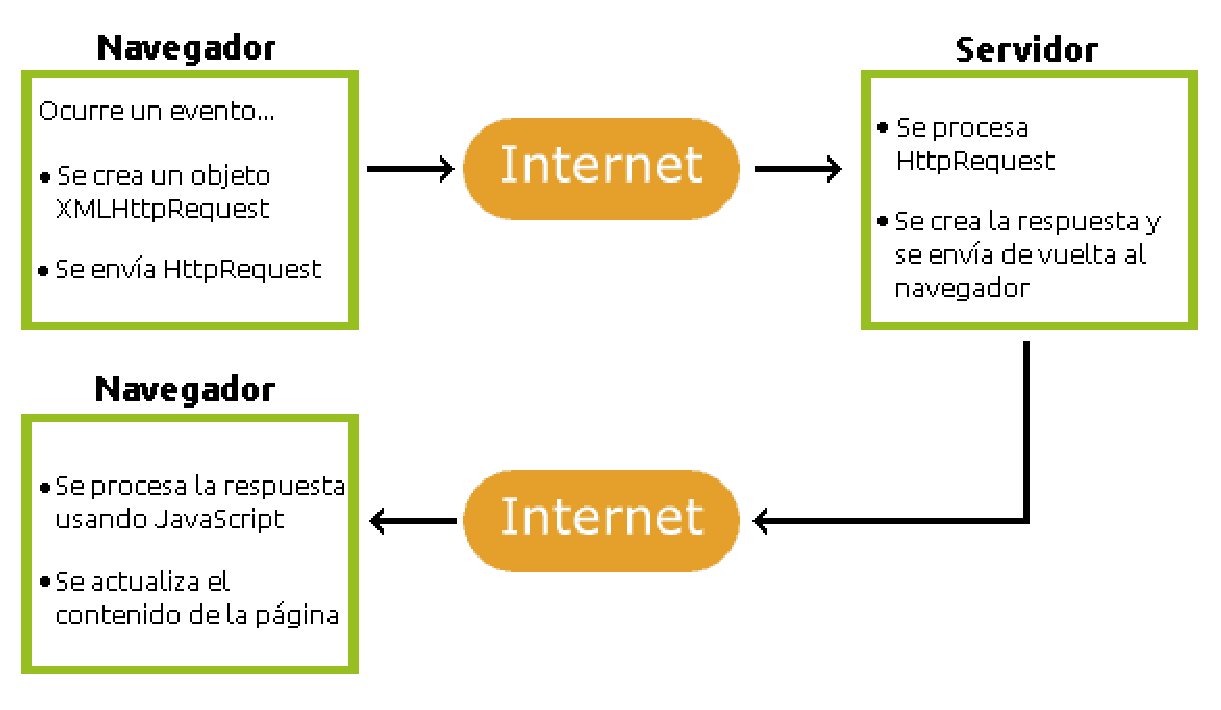
\epsfig{file=imagenes/ajax.eps,width=5.28in}
\caption{Funcionamiento de Ajax.}
\label{fig:ajax}
\end{figure}

Curiosamente, la primera aplicación Ajax que alcanzó la popularidad a nivel
mundial fue Google Suggest (las sugerencias del conocido buscador, lanzadas en
diciembre de 2004), y este ha sido precisamente uno de los usos que se le ha
dado en el marco de este proyecto: sugerir proyectos y clientes que listados de
otro modo resultarían demasiado pesados. La otra parte de la herramienta que
hace uso intensivo de Ajax es el buscador global.

Además, Ajax a pesar de ser una tecnología relativamente reciente, no solo es
compatible con los navegadores modernos, sino que también está soportado en IE5
e IE6, gracias a una implementación particular del objeto HttpRequest que estos
navegadores ya incluían.

\begin{lstlisting}
var xmlhttp;
if (window.XMLHttpRequest)
  {// codigo para IE7+, Firefox, Chrome, Opera, Safari
  xmlhttp=new XMLHttpRequest();
  }
else
  {// codigo para IE6, IE5
  xmlhttp=new ActiveXObject("Microsoft.XMLHTTP");
  }
\end{lstlisting}

\section{Librerías}

El uso de librerías forma parte del día a día del desarrollo web y de la
programación en general. En este caso se han usado dos librerías básicas y de
naturaleza muy distinta, una librería de JavaScript y otra PHP. Además, la
aplicación ya contaba con una librería para la selección de fechas en formato
calendario, pero debido a que ya estaba en uso y a su simplicidad, no se
describirá.

\subsection{Sorttable}

\textit{Sorttable}\footnote{Sitio oficial de la librería:
\href{http://www.kryogenix.org/code/browser/sorttable/}{
kryogenix.org/code/browser/sorttable/}} es una librería (o minilibrería)
JavaScript que permite la ordenación de filas de tablas una vez cargadas y sin
necesidad de recargar la página. El uso de esta librería no responde a una
necesidad específica, pero, de acuerdo con el cliente, la capacidad para ordenar
cualquier tabla según el tipo de dato que contengan es una de las cosas que más
se echan de menos en las aplicaciones web en contraste con las aplicaciones de
escritorio.

Una de las formas más comunes de resolver esta carencia es
recargando la página pasándole al servidor la información acerca de como desean
ordenarse los datos. Sin embargo, gracias al uso de JavaScript, podemos lograr
este mismo resultado sin recargar la página y sin consumir recursos del lado
del servidor siguiente unas pautas muy sencillas acerca del buen formato de la
tabla: es necesario usar bloques de cabecera, cuerpo y pie de tabla:
\verb|<thead>|, \verb|<tbody>| \verb|<tfoot>|).

La librería es capaz de ordenar automáticamente los tipos de datos más comunes,
pero si se necesitan ordenar tipos de fecha complejos o personalizados (fechas
en formatos especiales), también ofrece la opción de ordenar por criterios
transparentes al usuario y distintos a lo que se ve en la tabla. Así, por
ejemplo, si se desea que ordene los meses pero los estamos mostranto en formato
texto (enero-diciembre), simplemente tendríamos que pasarle la información en
formato 1-12 a través del atributo \verb|sorttable_customkey|.

Finalmente, el usuario solo tendrá que pinchar sobre la cabecera de la columna
para reordenar las filas.

Es importante resaltar que la librería tiene licencia X11 del
\textit{Massachusetts Institute of Technology }(MIT), que autoriza su uso sin
restricciones con la condición de incluir el (breve) texto de la
licencia\footnote{La licencia completa puede consultarse aquí:
\href{http://www.xfree86.org/3.3.6/COPYRIGHT2.html}{
xfree86.org/3.3.6/COPYRIGHT2.html}} allá donde sea usada.

\subsection{PHPExcel}

PHPExcel\footnote{Sitio oficial de la librería:
\href{http://www.phpexcel.net}{
phpexcel.net}} es una poderosa librería que
proporciona un conjunto de clases PHP que permiten la lectura y escritura de
documentos Excel (2010 y anteriores). Incluye opciones para el manejo de
metadatos, estilos, múltiples hojas de cálculo, congelación de paneles, cálculo
de fórmulas Excel... La imagen \ref{fig:ejemplo_PHPExcel} representa algunas de
las cosas que se pueden conseguir con el uso de esta librería.

Esta librería se ha usado para exportar informes complejos en relación a la
asignación de horas de los empleados. Como se indicó en la sección
\ref{sec:requisitos_informes} sobre los requisitos de los informes, se
determinó que era importante conservar la funcionalidad anterior --el registro
de la distribución de horas se realizaba en hojas de cálculo--, por lo que se
creó la opción de exportar un resumen de la participación de los empleados en
todos los proyectos de la empresa (veáse la figura
\ref{fig:resumen_horas_asignadas_proyectos} del Manual de Usuario).

\begin{figure}
\centering
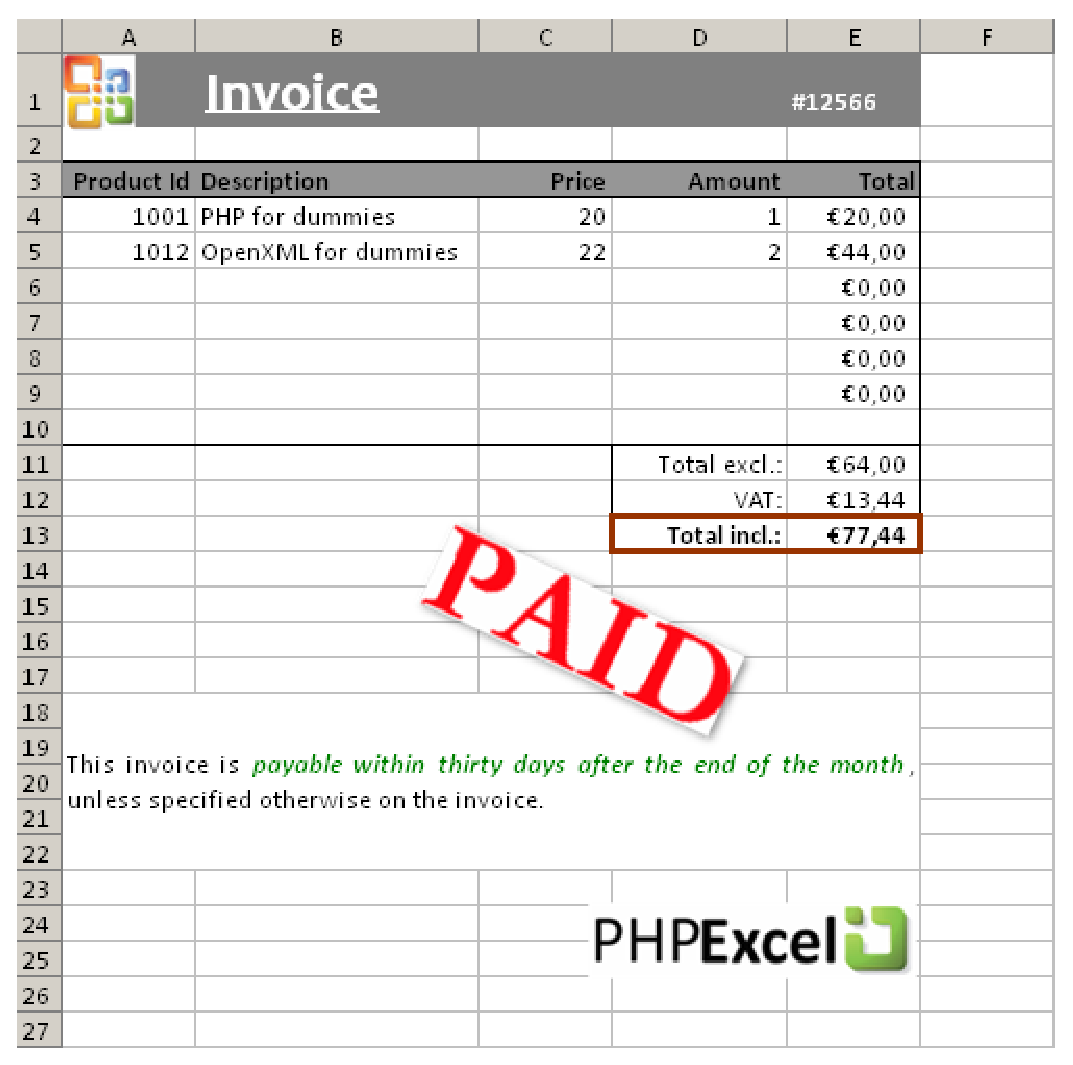
\epsfig{file=imagenes/ejemplo_PHPExcel.eps,width=3.5in}
\caption{Ejemplo de hoja de cálculo compleja.}
\label{fig:ejemplo_PHPExcel}
\end{figure}

El manejo de esta librería no es sencillo y requirió de un periodo de estudio
de aproximadamente una semana, pero el nivel de detalle de la documentación
facilitó enormemente esta tarea.

Por último, dejar constancia de que la librería tiene una licencia
LGPL\footnote{La licencia completa puede consultarse aquí:
\href{http://www.gnu.org/licenses/lgpl.html}{
gnu.org/licenses/lgpl.html}} (GNU
Lesser General Public License), que permite su uso libre pero no la
modificación del Software.

\subsection{JQuery}

La popularidad de JQuery\footnote{Sitio oficial de la librería:
\href{http://jquery.com/}{
jquery.com}} hizo que tanto el cliente como el
proyectante se interesasen por las posibilidades de esta librería de JavaScript,
por lo que fue estudiada con relativa profundidad. Finalmente, se decidió no
incluirla en el marco de este proyecto, pero el nuevo conocimiento adquirido
sería usado en otros desarrollos, como se explica más adelante en el capítulo
\ref{chp:conclusiones}.

\section{Detalles de la implementación. Algoritmos representativos}

\subsection{Distribución de horas por mes}
\label{sec:algoritmo_distribucion}

La asignación de horas debe seguir los requisitos funcionales descritos en la
sección \ref{sec:requisitos_gestion_horas}. Para facilitar la labor del lector,
se copia a continuación el punto que hace referencia a la distribución de las
horas:

\begin{quote}
La asignación de horas a un periodo se repartirá internamente por meses (no
días), de manera que las horas asignadas a un periodo que comprenda dos meses o
más se repartirán porcentualmente teniendo en cuenta el número de días
laborables de cada mes, y cuando sea posible, en múltiplos de 5. Debido a la
excesiva complejidad que se añadiría, no se tienen en cuenta las horas del
empleado en otros proyectos en el momento de la asignación.
\end{quote}

Secuencia de la distribución:
\begin{enumerate}
\item En primer lugar, debemos recoger los datos necesarios para realizar la
asignación, que llegan a partir del formulario de asignación (veáse la figura
\ref{fig:form_asig_horas} del Manual de Usuario). Estos datos son:

  \begin{itemize}
  \item Identificador del empleado.
  \item Identificador de la actividad.
  \item Tipo de horas (presentadas, aprobadas, justificadas).
  \item Fecha de inicio de la asignación.
  \item Fecha de fin de la asignación.
  \item Número de horas a distribuir.
  \item Descripción de la labor del empleado.
  \end{itemize}

\item Ahora se deben introducir los datos de la asignación en la tabla
PERSONAL\_ACTIVIDAD:

\begin{lstlisting}
INSERT INTO personal_actividad
(id_personal,id_actividad,f_ini,f_fin,descripcion)
VALUES
('$personal','$actividad','$f_ini_unix','$f_fin_unix','$descripcion')";
\end{lstlisting}

\item Se calculará el número de días laborables entre las dos fechas:

\begin{lstlisting}
function laborables($f_ini_unix,$f_fin_unix) {
	$current_date = $f_ini_unix; 
	$num = 0;
	while ($current_date <= $f_fin_unix) {
		$dia = date('w',$current_date);
		if ($dia > 0 && $dia < 6 &&
!esFestivoNacional(date('j',$current_date), date('n',$current_date))) {
			$num++;
		}
		$current_date += 86400;
	}
	return $num;
}
\end{lstlisting}

\textit{Nota: De hecho, esta función, que estuvo en funcionamiento durante meses
sin que el proyectante advirtiera ninguna anomalía, es incorrecta, como se
advertiría gracias a un plan de pruebas que se describirá en el capítulo
\ref{chp:pruebas}.}

\item A partir del número de días, se calculará la asignación de horas diaria
de forma proporcional, corrigiendo los excesos (se corrigen los excesos
provocados por la propia actividad, no en combinación con otras). Asimismo, se
calculará el número de meses completos (quitando los extremos) y de años
implicados en la asignación:

\begin{lstlisting}
$horas_dia = $duracion_en_horas / $duracion_en_dias;
if ($horas_dia > 8) {
	$horas_dia = 8;
}
$num_anios = $anio_fin - anio_inicio;
$num_meses_completos = ($num_anios * 12) + ($mes_fin - $mes_inicio) - 1;
\end{lstlisting}

Nótese que si solo hay un mes implicado en la asignación, el número de meses
completos se considerará, por convención, -1, y en este caso, se asignarán
todas las horas a ese mes, de nuevo, corrigiendo al máximo si hay exceso:

\begin{lstlisting}
if ($num_meses_completos == -1){
	$horas_aux = $duracion_en_horas;
	if($horas_aux > $duracion_en_dias * 8) {
		$horas_aux = $duracion_en_dias * 8;
	}
}
\end{lstlisting}

\item Si hay más de un mes implicado en la asignación, calculamos el número de
días laborables del primer mes desde la fecha de inicio hasta el final del mes,
y multiplicamos esos días por el número de horas que era necesario trabajar al
día según el número de días laborables global. Después, en el primer mes,
aumentamos el número de horas hasta el primer múltiplo de 5 siempre que el
valor de horas sea mayor que 5; si no, simplemente redondeamos al alza el número
de horas para el mes. Finalmente, comprobamos que no nos pasamos del máximo
posible ni de lo deseado y restamos el número de horas del mes al valor de horas
global para seguir con los meses siguientes.

\begin{lstlisting}
$laborables =
laborables($f_ini_unix,mktime(23,59,59,$mes_inicio+1,0,$anio_inicio));
$horas_aux = $horas_dia * $laborables;
if($horas_aux > 5) {
	$horas_aux = ceil($horas_aux / 5) * 5;
} else {
	$horas_aux = ceil($horas_aux);
}
if($laborables * 8 < $horas_aux)
	$horas_aux = $laborables * 8;
if($duracion_en_horas < $horas_aux)
	$horas_aux = $duracion_en_horas;
$duracion_en_horas -= $horas_aux;
\end{lstlisting}

\item Para los meses intermedios (lo que se llamó antes meses completos),
empleamos un bucle \verb|for| , ya que conocemos el mes inicial y el número de
meses completos. Así, calcularemos el número de días laborables del mes al que
se van a asignar las horas en cada caso y, como antes, se multiplicarán por la
asignación diaria prevista. Si dicha asignación es mayor que 5, se aumentarán
hasta el primer múltiplo de 5, y si no, solamente hasta el primer entero. Dado
que estamos redondeando al alza, haremos las comprobaciones pertinentes para no
pasarnos de la asignación global deseada ni de la asignación del mes máxima.
Finalmente, restaremos el valor obtenido al global a asignar:

\begin{lstlisting}
for ($mes_actual = $mes_inicio; $mes_actual < $mes_inicio +
$num_meses_completos; $mes_actual++) {
	$fecha_aux = mktime(0,0,0,$mes_actual + 1,1,$anio_inicio);
	$laborables = laborables($fecha_aux,mktime(0,0,0,$mes_actual +
2,0,$anio_inicio));
	$horas_aux = $horas_dia * $laborables;
	if($horas_aux > 5) {
		$horas_aux = ceil($horas_aux / 5) * 5;
	} else {
		$horas_aux = ceil($horas_aux);
	}
	if($laborables * 8 < $horas_aux)
		$horas_aux = $laborables * 8;
	if($duracion_en_horas < $horas_aux)
		$horas_aux = $duracion_en_horas;
	$duracion_en_horas -= $horas_aux;
}
\end{lstlisting}

\item Y para acabar todo el proceso, debemos introducir en el último mes todas
las horas que no hayan sido asignadas, asegurándonos que no son excesivas para
el mes (aunque sería extraño, ya que se han ido adelantando horas en los meses
intermedios).

\begin{lstlisting}
$laborables = laborables(mktime(0,0,0,$mes_fin,1,$anio_fin),$f_fin_unix);
$horas_aux = $duracion_en_horas;
if($laborables * 8 < $horas_aux)
	$horas_aux = $laborables * 8;
\end{lstlisting}

\end{enumerate}

\subsection{Horas ocupadas de un empleado en un mes}

Para llevar un control exhaustivo de la consistencia de los datos de cada
empleado, debemos ser capaces de calcular el número de horas que tiene asignadas
en un mes concreto (y por extensión, en años concretos). En general, una
información así requeriría una simple consulta a la base de datos, pero en el
momento en que se introduce el concepto de estado del proyecto, el proceso se
complica. Al igual que se hizo en la sección anterior, se reproduce a
continuación el punto de los requisitos funcionales que hace mención a este
cálculo:

\begin{quote}
Debe ser posible visualizar cuántas horas tiene asignadas un recurso en
cada uno de sus registro anuales, así como el total de horas libres (sin
asignar hasta el total de su convenio). El concepto de total de horas asignadas
se define como la suma de los siguientes valores:
 
\begin{enumerate}
\item En los proyectos en fase de presentación, las horas presentadas aunque
sean cero, siempre que no se hayan imputado horas aprobadas o justificadas. En
el último caso, se tomarán las de la fase más avanzada.

\item En los proyectos en fase de aprobación, las horas aprobadas aunque sean
cero, siempre que no se hayan comenzado a imputar horas justificadas.

\item En proyectos justificados o concluidos, las horas justificadas aunque
sean cero.
\end{enumerate}

Obviamente, un recurso puede tener horas asignadas en cada uno de los tres
tipos de estados.
\end{quote}

Para resolver el problema, se hará una consulta a la base de datos de forma que
se obtengan las horas asignadas al empleado desglosadas por meses y actividades:
\begin{lstlisting}
SELECT estado,
	horas,
	horas_aprobadas,
	horas_justificadas
FROM personal_horas ph join actividad ac on 
	ph.id_actividad=ac.id join proyectos pr on 
	ac.proyecto=pr.id
WHERE ph.id_personal=$id_personal and 
	ph.anio=$anio and 
	ph.mes=$mes
\end{lstlisting}

No se pueden agrupar las horas por proyectos ni por estado de esos
proyectos porque puede haber meses sueltos en los que a pesar de que el estado
del proyecto sea presentado, el empleado tenga horas aprobadas o justificadas, y
de acuerdo a los requisitos, esas son las que deben contarse para llevar una
cuenta más real. Entonces, para cada fila devuelta, se comprobará que horas hay
que escoger:

\begin{lstlisting}
$horas_ocupadas = 0;
for ($i = 0; $i < $numero_de_filas; $i++) {
	if ($filas[$i]['horas_justificadas'] != 0 ||
		$filas[$i]['estado'] == "JUSTIFICADO" ||
		$filas[$i]['estado'] == "CONCLUIDO")
	{
		$horas_ocupadas += $filas[$i]['horas_justificadas'];
	}
	elseif ($filas[$i]['horas_aprobadas'] != 0 || 
		$filas[$i]['estado'] == "APROBADO")
	{
		$horas_ocupadas += $filas[$i]['horas_aprobadas'];
	}
	else {
		$horas_ocupadas += $filas[$i]['horas'];
	}
}
\end{lstlisting}

\subsection{Buscador}

En esta sección se revisarán los fundamentos del uso de Ajax para conseguir el
efecto de búsqueda instantánea. Una vez activo el cuadro de texto del buscador,
se usa el evento \verb|onkeyup| para llamar, cada vez que se presione una tecla,
a una función de JavaScript \verb|mostrarResultados(...)|,

\begin{lstlisting}
function mostrarResultados(elt,ini) {
	var q = elt.value;
	showHint(q,"searchResults","buscador",ini);
	document.getElementById("buscando").src=
		"imagenes/loading.gif";
	document.getElementById('searchResults').style.opacity=
		'0.6';
	document.getElementById('searchResults').style.filter=
		'alpha(opacity=60)';
	if(q != "")
		document.getElementById("searchResults").style.display=
			"block";
	else
		document.getElementById("searchResults").style.display=
			"none";
}
\end{lstlisting}

que hace visible el contenedor de los resultados y disminuye su opacidad,
incluye una imágen que informa que el buscador está cargando y llama a su vez a
la función \verb|showHint(...)|:

\begin{lstlisting}
function showHint(str,elt,lista,ini) {
	if (str.length==0) {
	  document.getElementById(elt).innerHTML="";
	  return;
	}
	xmlhttp=GetXmlHttpObject();
	if (xmlhttp==null) {
	  alert ("Su navegador no soporta XMLHTTP!");
	  return;
	}
	var url="include/"+lista+".php";
	url=url+"?q="+str.trim();
	url=url+"&ini="+ini;
	url=url+"&sid="+Math.random();
	xmlhttp.onreadystatechange=stateChanged;
	xmlhttp.open("GET",url,true);
	xmlhttp.send(null);
}
\end{lstlisting}

\verb|showHint| crea un objeto HttpRequest como se indicó en la sección
\ref{sec:fundamentos_ajax}, donde se introdujo brevemente la tecnología. Ese
objeto se guarda en la variable \verb|xmlhttp|, que no se ha creado en esta
función sino que es una variable global. También en esta función se crea la
consulta con método \verb|GET| que se envía al archivo \verb|buscador.php| para
que este mande los resultados de la búsqueda de vuelta a JavaScript.

Esa respuesta es manejada por la función \verb|stateChanged|, que también
revierte los aspectos visuales a opacidad total, quita la imagen que indica que
el buscador está cargando... y lo hace de la siguiente manera:

\begin{lstlisting}
function stateChanged() {
	if (xmlhttp.readyState==4) {
	document.getElementById("searchResults").innerHTML=
		xmlhttp.responseText;
	document.getElementById("buscando").src="imagenes/not_loading.png";
	setTimeout("document.getElementById(
		 'searchResults').style.opacity='1'",0);
	document.getElementById('searchResults').style.filter=
		'alpha(opacity=100)';
	if(ir_arriba==1)
		window.scrollTo(currentXPosition(),0);
	else
		ir_arriba=1;
	}
}
\end{lstlisting}

\begin{quote}
\textit{Nota: para detalles específicos sobre la implementación de la
funcionalidad completa del buscador --paginación, búsqueda selectiva, número de
resultados por página y navegación por teclado--, se remite directamente al
código.}
\end{quote}

\subsection{Sobre la implementación de la base de datos}

La base de datos ha sido implementada usando la interfaz gráfica del
cliente MySQL-Front, que se reseñará brevemente en el apéndice
\ref{apx:software_utilizado}. Dado que el motor de almacenamiento empleado en el
resto de la base de datos era MyISAM, se siguó con la misma metodología, si
bien podría haberse combinado con otros motores como InnoDB. Hay
que tener en cuenta que al crear una tabla, MyISAM acepta (no da
error) la sintaxis de claves foráneas pero no las implementa\footnote{Como se
puede leer en la documentación oficial: \newline
\href{http://dev.mysql.com/doc/refman/5.1/en/ansi-diff-foreign-keys.html }{
dev.mysql.com/doc/refman/5.1/en/ansi-diff-foreign-keys.html}}.

Así, no se han aprovechado las ventajas de la cláusula \verb|ON DELETE| en
combinación con \verb|CASCADE| y se han tenido que implementar este tipo de
comprobaciones en los \textit{scripts} PHP. Por ejemplo, al borrar una
actividad, es necesario explicitar el borrado de toda la información que hace
referencia a esa actividad para no dejar la base de datos en un estado
inconsistente.







